\documentclass{beamer}

\usepackage{graphicx}
\usepackage{graphics}
\usepackage{amsmath,amssymb, amsfonts, mathtools}
%\usepackage{listings}

\usepackage{pgf}
\usepackage{tikz}
\usepackage[normalem]{ulem}
\usetheme{Data61}
\renewcommand{\t}[1]{\texttt{#1}}


\usepackage{amsmath}
\usepackage{amsfonts}
\usepackage{amssymb}
\usepackage{mathtools}
%\usepackage[usenames,dvipsnames,svgnames,table]{xcolor}
\usepackage{caption}

%%Found on Internet for Isabelle
% needed packages
\usepackage{verbatim}
\usepackage{pstricks,pst-node}
\usepackage{fancyvrb}
%\usepackage[fancyvrb]{listings}
\usepackage{listings}
% X-Symbols special characters
\DeclareTextSymbol{\textbackslash}{T1}{92}
\newcommand{\nsubset}{\not\subset}
%\newcommand{\textflorin}{\textit{f}}
\newcommand{\setB}{{\mathord{\mathbb B}}}
\newcommand{\setC}{{\mathord{\mathbb C}}}
\newcommand{\setN}{{\mathord{\mathbb N}}}
\newcommand{\setQ}{{\mathord{\mathbb Q}}}
\newcommand{\setR}{{\mathord{\mathbb R}}}
\newcommand{\setZ}{{\mathord{\mathbb Z}}}
\newcommand{\coloncolon}{\mathrel{::}}
\newcommand{\lsemantics}{\mathopen{\lbrack\mkern-3mu\lbrack}}
\newcommand{\rsemantics}{\mathclose{\rbrack\mkern-3mu\rbrack}}
\newcommand{\lcata}{\mathopen{(\mkern-3mu\mid}}
\newcommand{\rcata}{\mathclose{\mid\mkern-3mu)}}

% new language
\lstdefinelanguage{Isar}%
  {keywords={
        _first,theory,end,types,datatype,consts,defs,primrec,
        syntax,translations,apply,definition,fun,function, lemma,theorem,corollary,
        done,sorry,goal,proof,fixed variables,_last, inductive, where, if, then, else, where},
    keywordstyle=\color{Data61 light forest}\bfseries,
    keywordstyle=[3]\itshape,
        sensitive=true,
        morecomment=[l]{-- },
        literate=
                {\\<not>}{{$¬$}}1 {\\<times>}{{$×$}}1                 
                {\\<Rightarrow>}{{$\Rightarrow$}}1%
                {\\<equiv>}{{$\equiv$}}1 {~=}{{$\not=$}}1                         
                {\\<rightleftharpoons>}
                        {{$\rightleftharpoons$}}1
                {\\<exists>}{{$\exists$}}1
                {\\<parallel>}{{$\parallel$}}1
                {\\<Longrightarrow>}
                        {{$\Longrightarrow$}}1
                 {\\<lbrakk>}{{$\lsemantics$}}1
                {\\<rbrakk>}{{$\rsemantics$}}1
                {\\<longrightarrow>}
                        {{$\longrightarrow$}}1
                {\\<and>}{{$\land$}}1
                {\\<or>}{{$\lor$}}1
                {\\<bigwedge>}{{$\bigwedge$}}1
                {\\<forall>}{{$\forall$}}1
                {\\<langle>}{{$\langle$}}1
                {\\<rangle>}{{$\rangle$}}1
                {\\<models>}{{$\models$}}1
                {ü}{"u}1 {ä}{"a}1 {ö}{"o}1
                {Ü}{"U}1 {Ä}{"A}1 {Ö}{"O}1 {ß}{{ss}}1
  }[keywords,comments,strings]%

% useful defaults
\lstset{
  basicstyle=\footnotesize,
  commentstyle=\rm\it,
  flexiblecolumns=false,
  breaklines=true,
  breakautoindent=false
}

% possible usage
%\lstinline!apply(simp)!
%\begin{lstlisting}[language=Isar]{}
%datatype type = IntType | BoolType | FunType type type | ErrorType
%\end{lstlisting}
%\lstinputlisting[language=Isar]{foo.thy}

% Taken from Lena Herrmann at 
% http://lenaherrmann.net/2010/05/20/javascript-syntax-highlighting-in-the-latex-listings-package
\definecolor{lightgray}{rgb}{.9,.9,.9}
\definecolor{darkgray}{rgb}{.4,.4,.4}
\definecolor{purple}{rgb}{0.65, 0.12, 0.82}

\lstdefinelanguage{JavaScript}{
  keywords={typeof, new, true, false, catch, function, return, null, catch, switch, var, if, in, while, do, else, case, break, returns, contract},
  keywordstyle=\color{blue}\bfseries,
  ndkeywords={class, export, boolean, throw, implements, import, this},
  ndkeywordstyle=\color{darkgray}\bfseries,
  identifierstyle=\color{black},
  sensitive=false,
  comment=[l]{//},
  morecomment=[s]{/*}{*/},
  commentstyle=\color{purple}\ttfamily,
  stringstyle=\color{red}\ttfamily,
  morestring=[b]',
  morestring=[b]"
}

\lstset{
   extendedchars=true,
   tabsize=2,
   breaklines=true,
   captionpos=b
}


%%From Guillaume

\definecolor{pblue}{rgb}{0.13,0.13,1}
\definecolor{pgreen}{rgb}{0,0.5,0}
\definecolor{pred}{rgb}{0.9,0,0}
\definecolor{pgrey}{rgb}{0.46,0.45,0.48}

\lstset{%language=Java,
        showspaces=false,
        showtabs=false,
        breaklines=true,
        showstringspaces=false,
        breakatwhitespace=true,
%        commentstyle=\color{pgreen},
%       keywordstyle=\color{pblue},
%        stringstyle=\color{pred},
        basicstyle=\ttfamily,
%        stepnumber=1,
%        firstnumber=1,
%        linewidth=0.6\textwidth,
%        xleftmargin=0.2\textwidth,
%        xrightmargin=0.2\textwidth,
        numberfirstline=false}

\title[Towards Verifying Ethereum Smart Contract
Bytecode]{Towards Verifying Ethereum Smart Contract
	Bytecode in Isabelle/HOL}
\author[Myriam B\'{e}gel]{Myriam B\'{e}gel - \scriptsize{ENS Paris-Saclay, Universit\'{e} Paris-Saclay}}
\institute{joint work with Sidney Amani, Maksym Bortin, Mark Staples at Data61 (CSIRO)}
\date{January, 8th 2018}
\bibliographystyle{apalike}

\newlength{\textlarg}

%Tikz
\usetikzlibrary{arrows,automata}
\usetikzlibrary{positioning}
\tikzset{
	state/.style={
		rectangle,
		rounded corners,
		very thick,
		minimum height=2em,
		inner sep=2pt,
		text centered,
node distance=1.3cm,
	},
}
\renewcommand{\ULthickness}{2pt}

\newcommand{\stkout}[1]{
	\textcolor{Data61 green}{
		\ifmmode\text{\sout{\ensuremath{#1}}}
		\else\sout{#1}\fi}}

\newcommand{\triple}[3]{\{#1\}~#2~\{#3\}}
\newcommand{\Dtriple}[3]{\vDash\{#1\}~#2~\{#3\}}
\newcommand{\ttriple}[3]{[#1]~#2~[#3]}
\newcommand{\vinstr}{{\color{Data61 green}\vdash_\mathrm{instr}}}
\newcommand{\vblock}{{\color{Data61 plum}\vdash_\mathrm{block}}}
\newcommand{\vprog}{{\color{Data61 ocean blue}\vdash_\mathrm{prog}}}
\newcommand{\tinstr}[3]{\vinstr[#1]\:#2\:[#3]}
\newcommand{\tblock}[3]{\vblock[#1]\:#2\:[#3]}
\newcommand{\tprog}[4]{\mathit{#1}\vprog[#2]\:#3\:[#4]}

\newcommand{\defeq}{\mathrel{\stackrel{\mbox{\tiny \it def}}{=}}}
\newcommand{\subpred}{\Rightarrow}
\newcommand{\sconj}{\wedge^*}
%\newcommand{\coloncolon}{\mathrel{::}}
\newcommand{\pvalid}[3]{\models\{#1\}\:#2\:\{#3\}}
\newcommand{\tvalid}[3]{{\color{Data61 dark mint}\models}[#1]\:#2\:[#3]}
\newcommand{\ttrip}[5]{\mathit{#1} \vdash_{\mathrm{#2}}[#3]\:#4\:[#5]}
\newcommand{\xnext}{\mathit{next}}
\newcommand{\code}[1]{\mathit{code}(#1)}
\newcommand{\cont}{\mathit{continuing}}
\newcommand{\ncont}{\mathit{not\mbox{-}continuing}}
\newcommand{\pc}{\mathit{pc}}
\newcommand{\gaspred}{\mathit{gas\mbox{-}pred}}
\newcommand{\stackh}{\mathit{stack\mbox{-}height}}
\newcommand{\stack}{\mathit{stack}}
\newcommand{\storage}{\mathit{storage}}
\newcommand{\instr}[1]{\mathtt{#1}}
\newcommand{\pure}[1]{\langle#1\rangle}
\newcommand{\hd}{\mathit{head}\:}
\newcommand{\RuleL}[2]{\begin{array}{l}#1\\\hline\noalign{\smallskip}#2\end{array}}
\newcommand{\RuleC}[2]{\begin{array}{c}#1\\\hline\noalign{\smallskip}#2\end{array}}
\newcommand{\Rule}[2]{\dfrac{#1}{#2}}
\newcommand{\bblocks}{\mathit{build\mbox{-}blocks}}
\newcommand{\cblocks}{\mathit{connect\mbox{-}blocks}}
\newcommand{\fblock}{\mathit{first\mbox{-}block}}
\newcommand{\len}[1]{|#1|}
\newcommand{\wfblocks}{\mathit{wf\mbox{-}blocks}}
%Solidity
\lstset{
	basicstyle=\footnotesize,
	commentstyle=\rm\it,
	flexiblecolumns=false,
	breaklines=true,
	breakautoindent=false
}

\definecolor{lightgray}{rgb}{.9,.9,.9}
\definecolor{darkgray}{rgb}{.4,.4,.4}
\definecolor{purple}{rgb}{0.65, 0.12, 0.82}


\lstdefinelanguage{Solidity}{
	keywords={typeof, new, true, false, catch, function, return, null, catch, switch, var, if, in, while, do, else, case, break, returns, contract, public,payable},
	keywordstyle=\color{Data61 ocean blue}\bfseries,
	keywordstyle=[2]\color{black}\bfseries,
	keywordstyle=[3]\color{Data61 plum}\bfseries,
	keywordstyle=[4]\color{black}\bfseries,
	keywords=[2]{address, uint256},
	keywords=[3]{require,selfdestruct},
	keywords=[4]{address,uint256},
	ndkeywords={class, export, boolean, throw, implements, import, this},
	ndkeywordstyle=\color{black}\bfseries,
	numbers=left,
	numbersep=5pt,
	identifierstyle=\color{black},
	sensitive=false,
	comment=[l]{//},
	morecomment=[s]{/*}{*/},
	commentstyle=\color{purple}\ttfamily,
	stringstyle=\color{red}\ttfamily,
	morestring=[b]',
	morestring=[b]",
	escapeinside={@}{@},numbers=left,xleftmargin=2em
}

\begin{document}
%%1
\maketitle



%%2
\part{Context}
\frame{\partpage}

\begin{frame}{Cost of smart contract bugs}
	\includegraphics[scale=0.5]{Figures/intro.png}
\end{frame}

%%3
\begin{frame}{Ethereum}
	%\begin{columns}[c]
	%	\column{.6\textwidth}
		\begin{itemize}
			\item Decentralised platform (\emph{blockchain}) to run smart contracts, Turing-complete programs
			\item Smart contracts can receive/transfer cryptocurrency (\emph{ether})
			\item Smart contracts run by the \emph{Ethereum Virtal Machine}
			\item Critical use for: voting, pharmaceutical supply chains, electrical power grids
			\item No central authority
		\end{itemize}
	%	\column{.4\textwidth}
		\centering\includegraphics[scale=0.2]{Figures/ETHEREUM-LOGO_PORTRAIT_Black_small.png}
	%\end{columns}
\end{frame}

%%4
\begin{frame}{Ethereum Virtual Machine}
	\begin{columns}[c]
		\column{.6\textwidth}
		\begin{itemize}
			\item Stack: for instructions operands
			\item Memory: temporary variables
			\item Storage: persistent variables
			\item Environment variables
			\item Inter-contract calls
			\item High-level languages:
			Solidity, Viper, LLL, etc
		\end{itemize}
		\column{.4\textwidth}
		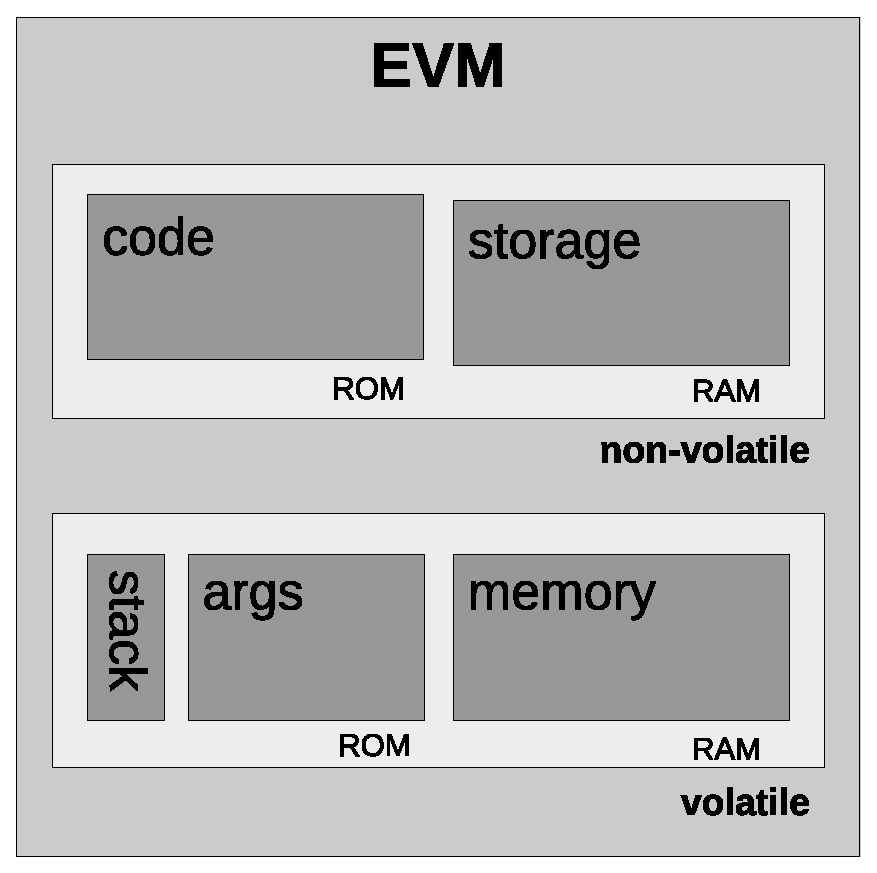
\includegraphics[scale=0.3]{Figures/evm.eps}
	\end{columns}
\end{frame}

%%5
\begin{frame}{EVM bytecode verification}
	\begin{itemize}
	    \item Yoichi Hirai formalised and validated EVM in Isabelle/HOL
	 
	    \item Reasoning about a flat, unstructured list of instructions is tedious
		\begin{itemize}
			\item Cannot match syntactically on program structure
		\end{itemize}
	
	    \item Our contributions:
	    \begin{itemize}
	    	\item Total correctness properties of contracts based on gas consumption
	    	\item Sound program logic to derive such properties
	    	\item Reasoning at the level of bytecode split into basic blocks
	    	\item Automation of verification condition generator
	    \end{itemize}
	\end{itemize}
\end{frame}

%%8
\part{Contributions}
\frame{\partpage}

\begin{frame}{Partial correctness statements}
	$\xnext$ = single machine step
	\\~\\
	\begin{center}
			$\pvalid{P}{c}{Q}$ iff \\
			$\forall s. F. (P \sconj \code{c} \sconj F)\:s \Rightarrow$ \\
			$\exists k. (Q \sconj \code{c} \sconj F)\:\xnext^k(s)$
	\end{center}

	~\\
	\uncover<2>{
	Does not ensure reaching a terminating state without the $\ncont$ flag. \\
	$\pvalid{P}{c}{\ncont \sconj Q'}$ means $c$ \emph{terminates} in a $Q'$-state}
\end{frame}

\begin{frame}{Total correctness statements}
	\begin{itemize}
		\item<1-> States with $\ncont$ are fixed-points of $\xnext$
		\item<2-> Every execution ends up in a terminating state: \\a smart-contract ends normally or runs out of gas
		\item<3-> $\xnext_\mu (s) = \xnext^k(s)$ where $\xnext^k(s)$ is the first iteration containing $\ncont$
	\end{itemize}
	\uncover<4->{
	\begin{center}
		$\tvalid{P}{c}{Q}$ iff \\
		$\forall s. F. (P \sconj \code{c} \sconj F)\:s \Rightarrow$ \\
		$(Q \sconj \code{c} \sconj F)\:\xnext_\mu(s)$
	\end{center}}
	\begin{itemize}
		\item<5-> $Q$ enforced to be terminating
	\end{itemize}
\end{frame}

%%9
\begin{frame}{Program logic}	
	3 levels for the program logic\\~
	\begin{itemize}
		\item<2-> For the instructions $\vinstr$
			\begin{itemize}
				\item one rule per instruction
%				\item<5-> non-terminating semantic with 1 step
			\end{itemize}
		\item<3-> For the \emph{basic blocks} $\vblock$
			\begin{itemize}
				\item unroll list of sequential instructions
%				\item<5-> non-terminating semantic with $n$ steps \\ $n=$ number of instructions
			\end{itemize}
		\item<4-> For the program $\vprog$
			\begin{itemize}
				\item jump from one block to another
%				\item<6-> terminating semantic
			\end{itemize}
	\end{itemize}
	\uncover<5>{
		\begin{figure}
			\vspace{-10pt}
			\[
			\dfrac
			{\dfrac
				{\dfrac{}{\tinstr{P}{hd~b}{R_1}}
					\quad
					\dfrac
					{\vdots}
					%{\dfrac{}{\vinstr \sim} \quad
					%	\dfrac{\dots}{\vblock \sim}}
					{\tblock{R_1}{tl~b}{R}}}
				{\tblock{P}{b}{R}}
				\quad \dfrac{\vdots}{\tprog{prog}{R}{b'}{Q}}}
			{\tprog{prog}{P}{b}{Q}}\]
		\end{figure}}
\end{frame}

\begin{frame}{Sequential block}
	Maximum block of straight-line code - Jumps are removed
	\\~\\
	\centering
	\begin{tabular}{c | r l | c}
		block index & address & instruction & block type\\
		\hline
		{0}&       0       &       $\instr{OR}$&\textit{Next}\\
		&       1       &       $\instr{ADD}$&\\
		&    2       &       $\instr{SWAP1}$&  \\
		\hline
		{3}&       3       &       $\instr{JUMPDEST}$&\textit{Jump}\\
		&       4       &       $\instr{MLOAD}$&\\
		&       5       &       $\instr{POP}$&\\
		&    \textcolor{gray}{6}     &       {\color{gray}$\instr{JUMP}$}& \\
		\hline
		{7}&       7       &       $\instr{DUP3}$&\textit{Jumpi}\\
		&       8       &       $\instr{PUSH1}\;0$&\\
		&       10      &       $\instr{ISZERO}$&\\
		&    \textcolor{gray}{11}    &       {\color{gray}$\instr{JUMPI}$}& \\
		\hline
		{12}&       12      &       $\instr{POP}$&\textit{Terminal}\\
		&   13      &       $\instr{RETURN}$& \\
		\hline
	\end{tabular}
\end{frame}

\begin{frame}{Rules for $\mathit{Terminal}$ and $\mathit{Next}$ blocks}
	\[
	\RuleC{\tblock{P}{\mathit{xs}}{Q}}
	{\tprog{prog}{P}{(n, \mathit{xs}, \mathit{Terminal})}{Q}}
	\]
	~\\
	\uncover<2->{
	\[
		\RuleC{\begin{array}{l} \tblock{P}{\mathit{xs}}{\pc\;\textcolor<3->{Data61 vermillion}{m} \sconj R} 
		\\
		(\textcolor<3->{Data61 vermillion}{m}, \mathit{ys},t) \in \mathit{blocks} 
		\\
		\tprog{prog}{\pc\;\textcolor<3->{Data61 vermillion}{m} \sconj R}{(\textcolor<3->{Data61 vermillion}{m}, \mathit{ys},t)}{Q}
		\end{array}}
	{\tprog{prog}{P}{(n, \mathit{xs}, \mathit{Next})}{Q}}
	\]}
\end{frame}

%%14
\begin{frame}{Rule for a Jump block}
	\[
	\RuleC{\begin{array}{l}\tblock{P}{\mathit{xs}}{R_1} \\
			(j, \mathit{ys},t) \in \mathit{blocks} \\
			\hd\mathit{ys} = (j, \instr{JUMPDEST}) \\
			\tprog{\mathit{blocks}}{R_2}{(j, \mathit{ys},t)}{Q}
		\end{array}}
		{\tprog{\mathit{blocks}}{P}{(n, \mathit{xs}, \mathit{Jump})}{Q}}
	\]
	\uncover<2->{
		\begin{align*}
		R1 = ~& {\color{Data61 plum}\langle h \leq 1023 \wedge \color{Data61 plum}8 \leq g \rangle}~ \wedge^* 
		{\color{Data61 dark mint}\texttt{continuing }} \wedge^*
		{\color{Data61 ocean blue}\texttt{gas-pred g }} \wedge^*\\
		&{\color{Data61 vermillion}\texttt{program-counter (n + size xs) }}\wedge^*\\
		&{\color{Data61 fuchsia}\texttt{stack-height (Suc h) }} \wedge^*
		{\color{Data61 fuchsia}\texttt{stack h j }} \wedge^*
		{\color{Data61 light forest}\texttt{rest}}\\
		R2 = ~&{\color{Data61 dark mint}\texttt{continuing }} \wedge^*
		{\color{Data61 ocean blue}\texttt{gas-pred (g - 8) }} \wedge^*\\
		&{\color{Data61 vermillion}\texttt{program-counter j }}\wedge^*
		{\color{Data61 fuchsia}\texttt{stack-height h }} \wedge^*
		{\color{Data61 light forest}\texttt{rest}}
		\end{align*}
	}
	\uncover<3>{Similar for JUMPI}
\end{frame}

\begin{frame}{Rules for a basic block}
	\[
	\RuleC{\begin{array}{l}\tinstr{P}{x}{R} \\
			\tblock{R}{\mathit{xs}}{Q}
		\end{array}}
		{\tblock{P}{x\mbox{::}\mathit{xs}}{Q}}
	\]
	~\\
	\uncover<2>{
		\[
		\RuleC{P \subpred Q} 
		{\tblock{P}{\mathit{Nil}}{Q}}\]
		}
\end{frame}

\begin{frame}{Example for an instruction}
	Rule for ADD
	\begin{align*}
	\vinstr&\\
	[&{\color<2>{Data61 plum}\langle h \leq 1023 \wedge 3 \leq g \rangle}~ \wedge^*\\
	&{\color<3>{Data61 dark mint}\texttt{continuing }} \wedge^*
	{\color<4>{Data61 vermillion}\texttt{program-counter n }} \wedge^*\\
	&{\color<5>{Data61 ocean blue}\texttt{gas-pred g }} \wedge^*
	{\color<6>{Data61 fuchsia}\texttt{stack-height (Suc (Suc h)) }} \wedge^*\\
	&{\color<6>{Data61 fuchsia}\texttt{stack (Suc h) a }} \wedge^*
	{\color<6>{Data61 fuchsia}\texttt{stack h b }} \wedge^*
	{\color<7>{Data61 light forest}\texttt{F}}]
	\\
	(&\texttt{\textcolor<4>{Data61 vermillion}{n}, \textcolor<1>{Data61 light teal}{ADD}}) \\
	[&{\color<3>{Data61 dark mint}\texttt{continuing }} \wedge^*
	{\color<4>{Data61 vermillion}\texttt{program-counter (n + 1) }} \wedge^*\\
	&{\color<5>{Data61 ocean blue}\texttt{gas-pred (g - 3) }} \wedge^*
	{\color<6>{Data61 fuchsia}\texttt{stack-height (Suc h) }} \wedge^*\\
	&{\color<6>{Data61 fuchsia}\texttt{stack h (a+b) }} \wedge^*
	{\color<7>{Data61 light forest}\texttt{F}}]
	\end{align*}
	\uncover<8>{Currently, 96/124 instructions specified}
\end{frame}

\begin{frame}{Soundness}
		\[
		\RuleC{\begin{array}{l}
			\tinstr{P}{x}{Q} \\
			(P \sconj \code{[x]} \sconj F)\: s
			\end{array}}
		{(Q \sconj \code{[x]} \sconj F)\: \xnext(s)}
		\]
		~\\
		\uncover<2->{	\[\RuleC{\begin{array}{l}
				\tblock{P}{\mathit{xs}}{Q} \\
				(P \sconj \code{\mathit{xs}} \sconj F)\: s
				\end{array}}
			{(Q \sconj \code{\mathit{xs}} \sconj F)\: \xnext^{\len{\mathit{xs}}}(s)}\]}
		~\\
		\uncover<3->{	\[
			\RuleC{\begin{array}{l}
				\tprog{\bblocks\: c}{P}{\fblock}{Q} \\
				0 < \len{c} < 2^{256} 
				\end{array}}
			{\tvalid{P}{c}{Q}}
			\]}
\end{frame}

\begin{frame}[fragile]{Case-study - Contract}
Escrow smart contract allowing an arbiter to clear\\
a transaction between two parties.\\
		\begin{lstlisting}[language=Solidity]
contract Escrow {
	@\label{lst:storevarbeg}@    address buyer;
	    address seller;
	    address arbiter;
	@\label{lst:storevarend}@    uint256 amount;
	
	@\label{lst:constbeg}@    function Escrow(address _buyer,
	    address _seller,
	    uint256 _amount) {
		@\label{lst:constreq}@        require (amount > 0);
		        buyer = _buyer;
		        seller = _seller;
		        arbiter = msg.sender;
		@\label{lst:constend}@        amount = _amount;
	    }
	    @\ldots@
	\end{lstlisting}
	\end{frame}
	
	\begin{frame}[fragile]{Contract}
		\begin{lstlisting}[language=Solidity]
contract Escrow {
    @\ldots@
    function addfund() payable public {
		@\label{lst:addfundbeg}@        require (amount > 0 &&
        msg.value == amount &&
		@\label{lst:addfundsender}@                 msg.sender == buyer);
		@\label{lst:addfundend}@        amount = 0;
    }
    function refund() public {
		@\label{lst:refundbeg}@        require (amount == 0 &&
        msg.sender == arbiter);
		@\label{lst:refundend}@        selfdestruct(buyer);
    }
    function pay() public {
		@\label{lst:paybeg}@        require (amount == 0 &&
        msg.sender == arbiter);
		@\label{lst:payend}@        selfdestruct(seller);
    }
}
		\end{lstlisting}
\end{frame}

\begin{frame}[fragile]{Specification}
\begin{lstlisting}[language=Isar,keywords={[3]{addfund\_hash,pay\_hash,refund\_hash,}}]{} 
definition 
  spec_Escrow :: [address, address, address, address, 
                  256 word, 32 word, 256 word]
                 \<Rightarrow> contract_action
where
  spec_Escrow sender buyer seller arbiter 
              amount hash value =
 (if hash = addfund_hash \<and> sender = buyer \<and>
     value = amount \<and> amount > 0 then
    ContractReturn []
  else if hash = refund_hash \<and>
          sender = arbiter \<and> value = 0 \<and>
          amount = 0 then
         ContractSuicide buyer
       else if hash = pay_hash \<and> sender = arbiter \<and>
               value = 0 \<and> amount = 0 then
              ContractSuicide seller
            else
              ContractFail [ShouldNotHappen])
		\end{lstlisting}
	\end{frame}
	
	\begin{frame}[fragile]{Specification}
		\begin{lstlisting}[language=Isar,keywords={[3]{addfund\_hash,pay\_hash,refund\_hash,}}]{} 
definition
  spec_amount :: [address, address, address, 256 word, 
                  32 word, 256 word] \<Rightarrow> 256 word
where
  spec_amount sender buyer seller amount hash value =
  (if hash = addfund_hash \<and> sender = buyer \<and>
             value = amount \<and> amount > 0 then
     0
   else
     amount)
\end{lstlisting}	
\end{frame}

\begin{frame}[fragile]{Correctness statement}
	\begin{lstlisting}[language=Isar,keywords={[3]{hash,sender,buyer,seller,arbiter,amount,v}}]{}
	theorem verify_escrow:
	  \<exists>r. \<models> [pc 0 \<and>* stack_height 0 \<and>*
	    sent_data (word_rsplit hash) \<and>*
	    sent_value v \<and>* caller sender \<and>*
	    memory_usage 0 \<and>* continuing \<and>*
	    gas_pred 40000 \<and>*
	    storage 0 (ucast buyer) \<and>*
	    storage 1 (ucast seller) \<and>*
	    storage 2 (ucast arbiter) \<and>*
	    storage 3 (ucast amount) \<and>*
	    ... ]
	  (build_blocks bytecode_Escrow)
	  [action (spec_Escrow sender buyer seller
	    arbiter amount hash v) \<and>*
	    storage 0 (ucast buyer) \<and>*
	    storage 1 (ucast seller) \<and>*
	    storage 2 (ucast arbiter) \<and>*
	    storage 3 (spec_amount sender buyer
	    seller amount hash v) \<and>* r]
	\end{lstlisting}
\end{frame}

\begin{frame}{Automation}
	\centering
	Syntaxic match to know which rule to apply
	\\~\\
	$\approx 40$ lines of proof for this example \\
	$\approx 500$ lines of reusable
	proof automation machinery
\end{frame}

%%19
\part{Future work}
\frame{\partpage}

%%20
\begin{frame}{Future work}
	\begin{itemize}
		\item Write \emph{sound} rules for all the instructions (36/70)
		\item Give more structure back (loops with heuristics)
		\item Restore functions calls
		\\~\\
		\begin{itemize}
			\item Proposal for EVM 1.5: static jumps and explicit function calls
		\end{itemize}
	\end{itemize}
\end{frame}


%%22
\frame[plain]{\thankspage{}{\scriptsize myriam.begel@ens-paris-saclay.fr}{}
	{Sidney Amani, Maksym Bortin, Mark Staples - \scriptsize Data61 (CSIRO)}
	{\scriptsize\textit{Firstname.Lastname}@data61.csiro.au}}

% \part \partpage not implemented yet
% thanks/question page not implemented

\bibliography{../bibli}

\end{document}